\documentclass{template/openetcs_article}
% Use the option "nocc" if the document is not licensed under Creative Commons
%\documentclass[nocc]{template/openetcs_article}
\usepackage {bsymb,b2latex}
\usepackage{lipsum,url,color}
\usepackage{float}

\usepackage{hyperref}

\usepackage{graphicx}


\graphicspath{{./template/}{.}{./images/}}
\begin{document}
\frontmatter
\project{openETCS}

%Please do not change anything above this line
%============================
% The document metadata is defined below

%assign a report number here
\reportnum{OETCS}



%---------------------------------------------------------

\newcommand{\true}{\ensuremath{true}}
\newcommand{\btext}[1]{{\it #1}}
\newcommand{\bvar}[1]{\btext{#1}}
\newcommand{\bevent}[1]{\btext{#1}}
\newcommand{\binv}[1]{\btext{#1}}
\newcommand{\bconst}[1]{\btext{#1}}
\newcommand{\bparam}[1]{\btext{#1}}
\newcommand{\bfunc}[1]{\btext{#1}}
\newcommand{\baxiom}[1]{\btext{#1}}
\newcommand{\btype}[1]{\btext{#1}}
\newcommand{\bguard}[1]{\btext{#1}}


% scaling for project creation wizard screenshots
\newcommand{\skalierung}{.6}

\title{Using Rodin with Projects on github}

\author{Matthias Güdemann\\Systerel, France}

% \date{}

% \begin{document}

% \maketitle

% define the coverart
\coverart[width=350pt]{chart}

\reporttype{Model Description}

%\begin{document}

\maketitle
\tableofcontents
\listoffiguresandtables
\newpage

\begin{abstract}
  This document gives a short introduction to Event-B modeling and the tool
  Rodin. It explains how Rodin projects on github can be imported into the Rodin
  platform. This is illustrated using the \texttt{model-evaluation} sub-project
  of \texttt{openETCS}.

  The document includes the documentation about how to install Rodin, lists the
  necessary plugins and suggests useful, additional plugins. At the end of this
  document, several frequently asked questions ({\bf FAQ}) and their respective
  answers are collected.
\end{abstract}

\section{Short Introduction to Event-B}
\label{sec:short-intr-event}

The formal language Event-B is based on a set-theoretic approach. It is a
variant of the B language, with a focus on system level
modeling~\cite{abrial-eventB-Book}. An Event-B model is separated into a static
and a dynamic part.

The dynamic part of an Event-B model describes abstract state machines. The
state is represented by a set of state variables. A transition from one state to
another is represented by parametrized events which assign new values to the
state variables. Event-B allows unbounded state spaces. They are constrained by
invariants expressed in first order logic with equality which must be fulfilled
in any case. The initial state is created by a special initialization event.

The static part of an Event-B model is represented by contexts. These consist of
carrier sets, constants and axioms. The type system of a model is described by
means of carrier sets and constraints expressed by axioms.

Event-B is not only comprised of descriptions of abstract state machines and
contexts, but also includes a modeling approach. This approach consists of
iterative refinement of the machines until the desired level of detail is
reached. In the Rodin tool, proof obligations are automatically created which
ensure correct refinement.

Together with the machine invariants, the proof obligations for the refinement
are formally proven, creating proof trees. To accomplish this, there are
different options: many proof obligations can be discharged by automated provers
(e.g., AtelierB, NewPP, Rodin's SMT-plugin), but as the underlying logic is in
general undecidable, it is sometimes necessary to use the interactive proof
support of Rodin.

Any external actions, e.g., mode changes by the driver or train level changes
are modeled via parametrized events. Only events can modify the variables of a
machine. An Event-B model is on the system level, events are assumed to be
called from a software system into which the functional model is embedded. The
guards of the events assure that any event can only be called when appropriate.

\section{Prerequisites}
\label{sec:prerequisites}

This section shortly describes the basic prerequisites to use Rodin projects on
github. First the installation of the Rodin platform itself, then the basic
plugins required to use the provided models and finally additional plugins which
facilitate usage and extension of the provided models.

\subsection{Rodin Platform}
\label{sec:rodin-platform}

This illustration uses the Rodin platform
2.7~\footnote{\url{http://www.event-b.org/}}, for general information on
Event-B, Rodin, various plugins etc. see the Event-B
Wiki~\footnote{\url{http://wiki.event-b.org/index.php/Main_Page}}. More details
on the installation on Rodin can be found
at {\url{http://www.event-b.org/install.html}}.

\subsection{Basic Plugins}
\label{sec:basic-plugins}

For plugin installations, it is recommended to tick the ``Contact all update
sites during install to fin required software'' (see
Figure~\ref{fig:plugin-install}). This will install all necessary dependencies
for each plugin, in case these are not yet installed.

\begin{figure}[ht]
  \centering
  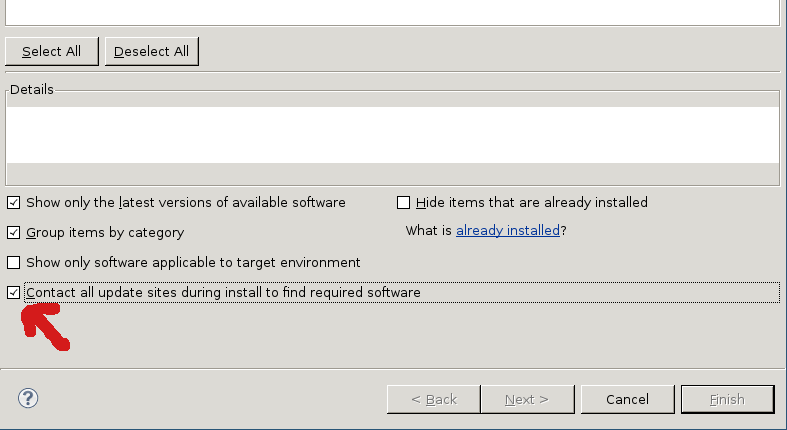
\includegraphics[width=.75\textwidth]{install-plugin}
  \caption{Plugin Installation}
  \label{fig:plugin-install}
\end{figure}

\paragraph{Provers}
\label{sec:atelier-b-provers}

The Atelier-B provers facilitate the construction of the proof trees for Rodin
proof obligations, by automatically discharging may proof obligations. Their
repository is available under Rodin as ``Atelier B Provers''.

Note, that these provers are not open source~\footnote{\url{
    http://www.atelierb.eu}}. Fully free provers are available, i.e., NewPP
which is installed by default and the SMT plugin prover
(see~\ref{sec:smt-solver-plugin}).

\paragraph{ProR Integration}
\label{sec:pror-integration}

The integration with ProR allows for the traceability of requirements in the
provided ReqIf files. The repository is available under Rodin as ``ProR'', where
the ``ProR Rodin integration feature'' must be installed. {\bf NOTE: } For the
current ProR version 0.6.1 there are known problems with Java version 6. It is
suggested to use Java version 7, if possible the latest JVM from
\url{http://www.oracle.com/technetwork/java/javase/downloads/jdk7-downloads-1880260.html}.

ProR is available under the EPL license.

\paragraph{EGit}
\label{sec:egit}

The integration with github is done via the EGit plugin. This plugin allows to
collaborate on Rodin models and to push/pull changes to github. The repository
is available under the official Eclipse repositories as ``Indigo Update Site''
where the ``Eclipse EGit'' must be installed.

EGit is available under the EPL license.

\paragraph{Model Decomposition}
\label{sec:model-decomposition}

The model decomposition plugin allows for structurization of Event-B
models. Larger models can be decomposed into smaller models with shared
variables or shared events. The decomposition keeps the correct proven
refinement relations and allows for independent refinement of the decomposed
machines. 

The model decomposition plugin is available under the EPL license.

\paragraph{iUML-B State Machines}
\label{sec:iuml-b-state}

The ``iUML-B State-Machines'' plugin allows for graphical modeling of
state-machines in an Event-B model. The state machines can be transformed into
Event-B code. It has a good integration with the ProB plugin which allows for
graphical animation of the machines.

The iUML plugin is available under the EPL license.

\subsection{Additional Plugins}
\label{sec:additional-plugins}

The additional plugins are not strictly necessary to analyze and inspect the
model. Nevertheless, it is suggested to install them if an extension of the
model is intended.

\paragraph{ProB / AnimB}
\label{sec:prob}

The ProB plugin provides means for model-checking and animation of Event-B
models. This requires finite instantiation of carrier sets and selection of an
initial state. In this situation, the plugin can verify deadlock freeness and
LTL formulas or can animate a system run. It is available from the ProB
repository under ``ProB for Rodin 2''.

AnimB also provides animation capabilities for Event-B machines. It is available
from the AnimB repository under ``AnimB''

ProB and AnimB are available under the EPL license.

\paragraph{SMT Solver Plugin}
\label{sec:smt-solver-plugin}

The SMT solver plugin will in general lead to a higher degree of automation for
the formal proofs. Experiments with industrial cases studies reduced the number
of non-automatically discharged proof obligations to one fourth. The plugin
comes bundled with two different solvers
(CVC3\footnote{\url{http://www.cs.nyu.edu/acsys/cvc3/}} and
veriT\footnote{\url{http://www.verit-solver.org/}}) and it can be extended with
various others, e.g., z3 from Microsoft or MathSAT5 from FBK. It is available
from the Rodin repository under ``SMT Solvers Integration''.

The SMT plugin is available under the EPL license.

\paragraph{Project Diagram}
\label{sec:project-diagram}

The project diagram plugin allows for visualization of the structure of a
model. In particular it visualizes the refinement relations between the
machines, the extension relation between the contexts and the sees relation
between machines and contexts. It is available from the Rodin repository under
``Event-B Project Diagram Plugin''.

\section{Importing Rodin Projects from github}
\label{sec:import-rodin-proj}

After the installation of Rodin and the necessary plugins, projects can be
imported from github into the local Rodin workspace. In the following, this is
explained using the Eclipse project creation wizard.

The first step is to select ``File $\rightarrow$ Import'' from the Eclipse menu
and then to select ``Git $\rightarrow$ Projects from Git'' as import source (see
Figure~\ref{fig:create-new-project}).

\begin{figure}[H]
  \centering
  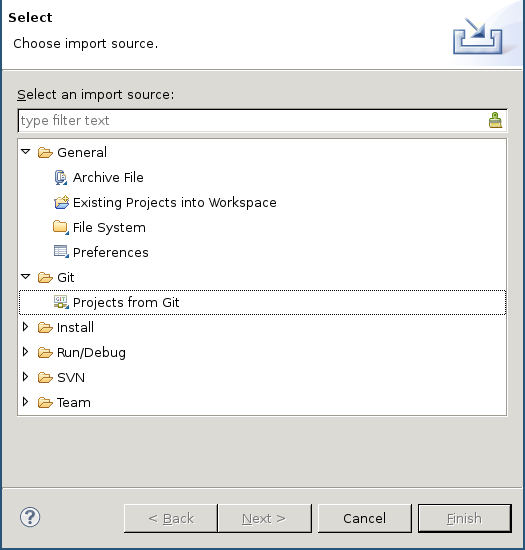
\includegraphics[width=\skalierung\textwidth]{project_import_step1}
  \caption{Creating a New Project}
  \label{fig:create-new-project}
\end{figure}

The next step is to specify where to find the git repository. For this, one has
to select the URI option as shown in Figure~\ref{fig:select-repo-source}.

\begin{figure}[H]
  \centering
  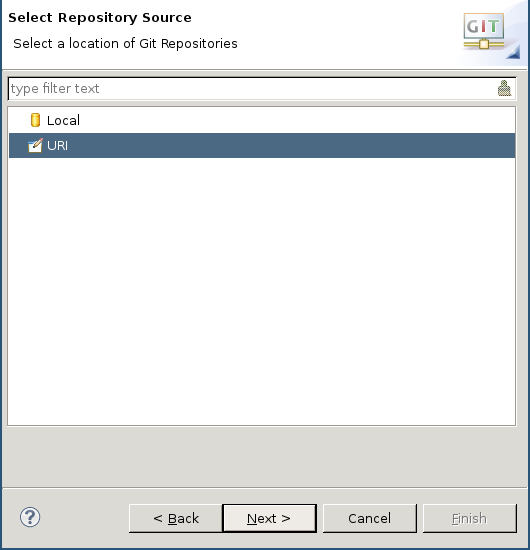
\includegraphics[width=\skalierung\textwidth]{project_import_step2}
  \caption{Selection of Repository Source}
  \label{fig:select-repo-source}
\end{figure}

The next step is to specify the URI of the repository on github. For the
model evaluation project, this is
\url{https://github.com/openETCS/model-evaluation.git}. This step also requires
the specification of the authentication data, i.e., the username and password
for github (see Figure~\ref{fig:specify-git-repo}).

\begin{figure}[H]
  \centering
  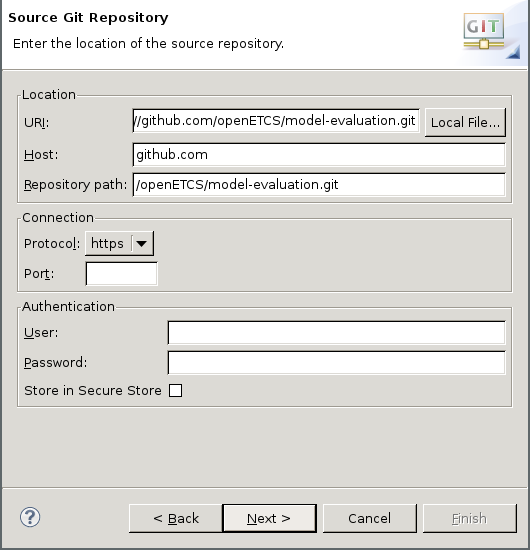
\includegraphics[width=\skalierung\textwidth]{project_import_step3}
  \caption{Specify github Repository}
  \label{fig:specify-git-repo}
\end{figure}

The next step is to select the desired branch of the repository. If in doubt and
there is more than one branch, selecting the ``master'' branch, as shown in
Figure~\ref{fig:select-branch} should be ok.

\begin{figure}[H]
  \centering
  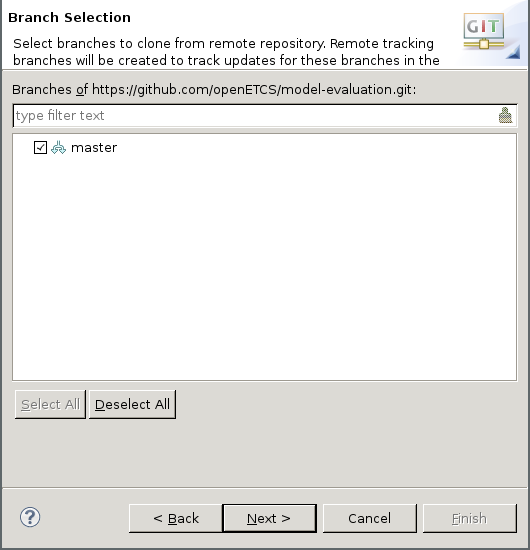
\includegraphics[width=\skalierung\textwidth]{project_import_step4}
  \caption{Select Branch of Repository}
  \label{fig:select-branch}
\end{figure}

For a local copy of the repository on github, an empty directory on the local
machine must be selected (or created) and a name of the remote repository can be
specified, the default is ``origin'' (see Figure~\ref{fig:local-copy}).

\begin{figure}[H]
  \centering
  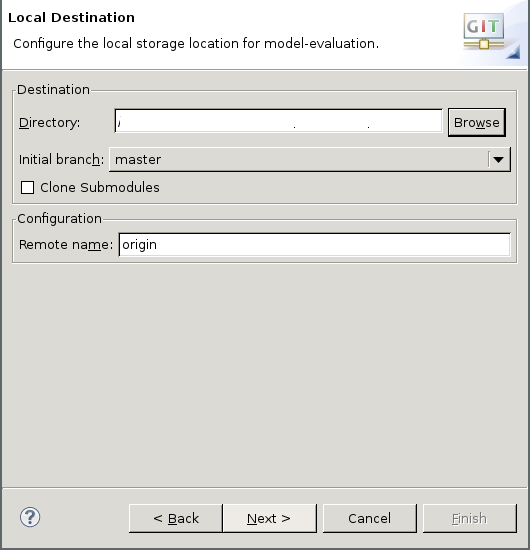
\includegraphics[width=\skalierung\textwidth]{project_import_step5}
  \caption{Local Repository Copy}
  \label{fig:local-copy}
\end{figure}

As there can be multiple projects in a repository, e.g., from different tools as
for the model-evaluation project, the correct one must be selected. To achieve
this, the collapsed directory tree as shown in
Figure~\ref{fig:select-project-import} must be expanded\footnote{Sometimes the
  information which directories are available is not shown directly (the
  collapse / expand symbol is lacking besides the ``working directory''). In
  this case it helps to push the ``back'' button to the previous window and
  return with ``next''.}.

\begin{figure}[H]
  \centering
  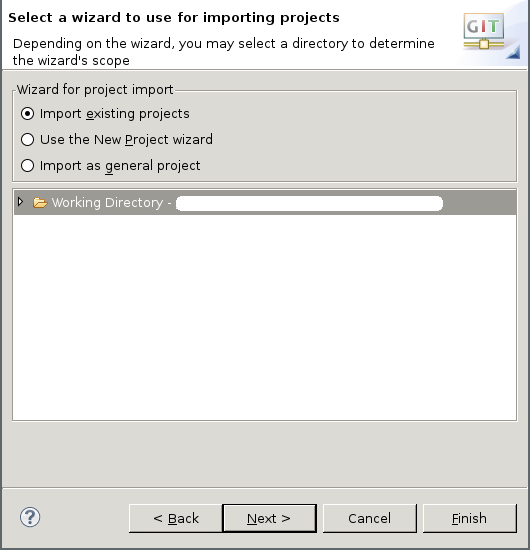
\includegraphics[width=\skalierung\textwidth]{project_import_step6}
  \caption{Select Project to Import}
  \label{fig:select-project-import}
\end{figure}

In the expanded tree, the project root directory of the project must be selected
as shown in Figure~\ref{fig:expanded-tree}.

\begin{figure}[H]
  \centering
  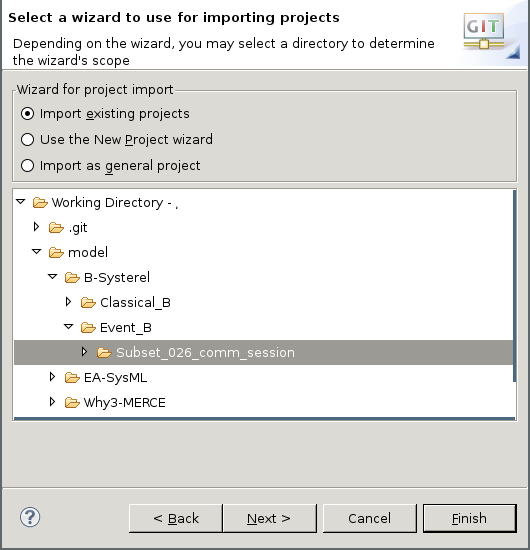
\includegraphics[width=\skalierung\textwidth]{project_import_step7}
  \caption{Expanded Directory Tree}
  \label{fig:expanded-tree}
\end{figure}

Once the correct directory has been selected, the contained projects can be
selected as shown in Figure~\ref{fig:import-project-workspace} and imported into
the local Rodin workspace.

\begin{figure}[H]
  \centering
  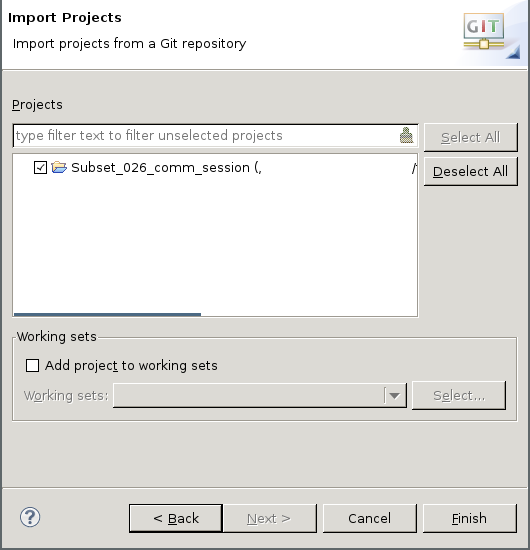
\includegraphics[width=\skalierung\textwidth]{project_import_step8}
  \caption{Import Project into Workspace}
  \label{fig:import-project-workspace}
\end{figure}

Once the project is imported into the workspace, it will appear in the Event-B
project explorer. There it can be updated to the current revision on the git
repository be right-clicking on the project and selecting ``Team $\rightarrow$
Pull''. 

\section{Frequently Asked Questions - FAQ}
\label{sec:faq}

\subsection{How are requirements traced?}
\label{sec:how-are-requirements}

For requirements tracing we use the ProR
plugin~\footnote{http://wiki.event-b.org/index.php/ProR} from
formalmind~\footnote{http://www.formalmind.com}. It is based on the OMG
standardized ReqIf format. It allows for tracing of Event-B modeling artifacts
in ReqIf files. Changes in either the model or the ReqIf are marked
automatically, the ProR view of Rodin is shown in Figure~\ref{fig:req-tracing}.


\begin{figure}[H]
  \centering
  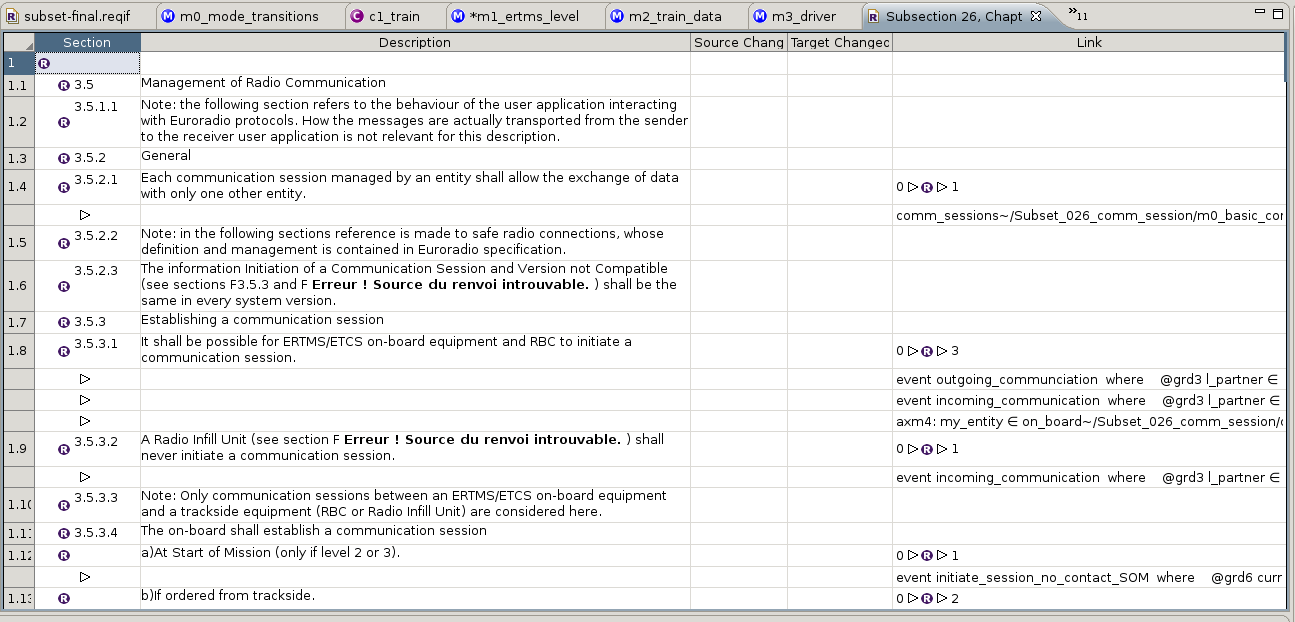
\includegraphics[width=\textwidth]{ReqIfinRodin}
  \caption{Requirements Tracing with ProR}
  \label{fig:req-tracing}
\end{figure}

To open a ReqIf file, the ``Resources'' view of Rodin must be selected which
will show all files in the project in the Project-Explorer.

\subsection{Proof obligations are not shown in the Event-b explorer. How to
  create them?}
\label{sec:proof-oblig-are}


This can have different causes. Trivial proof obligations are not shown, this
concerns in particular proofs for well-definedness~\footnote{see
  \url{http://handbook.event-b.org/current/html/well_definedness_proof_obligations.html}}. It
is also possible to hide proven proof obligations by toggling the green button
on top of the Event-B Explorer shown in
Figure~\ref{fig:tree-proof-obligations} (button is inactive in this example).

\begin{figure}[H]
  \centering
  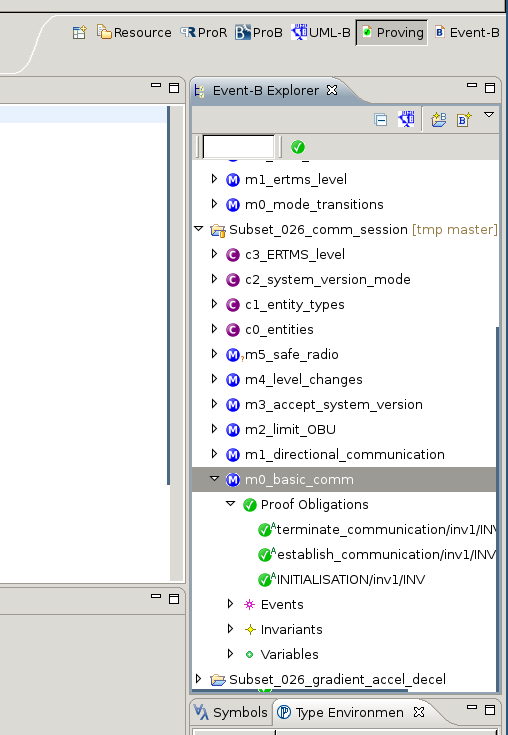
\includegraphics[width=.5\textwidth]{RodinEventBView}
  \caption{Event-B Project Tree View with Proof Obligations}
  \label{fig:tree-proof-obligations}
\end{figure}

Another possibility is a problem with some installed plugins, in this case the
project can be cleaned by selecting ``Project->Clean'' from the main Rodin
menu. If  ``Project->Build Automatically'' is selected the project will be
automatically refreshed, this is also possible manually by selecting the
project, hitting F5 or selecting ``Refresh'' from the right-click menu.

\subsection{If I try to open a ReqIf file, Rodin nothing happens and Rodin
  freezes. What happened?}
\label{sec:if-i-try}

There is a problem in the ProR plugin which can cause this behavior (e.g., see
here \url{https://bugs.eclipse.org/bugs/show_bug.cgi?id=397672}). Currently
the best solution is to install the most recent JDK
from~\url{http://www.oracle.com/technetwork/java/javase/downloads/jdk7-downloads-1880260.html}.

\subsection{How can I see the definition of an Event-B model artifact which is
  linked in a ReqIf file?}
\label{sec:how-can-i}


When opening a ReqIf file, the standard view only displays whether a
requirement is linked or not. To see all linked model elements, the
``SpecRelations (Links)'' button must be toggled (see
Figure~\ref{fig:spec-relations-button}).

\begin{figure}[H]
  \centering
  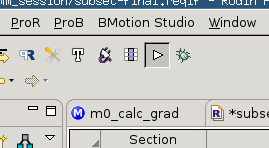
\includegraphics[width=.35\textwidth]{ProR-Link-Toggle}
  \caption{Active SpecRelations Button}
  \label{fig:spec-relations-button}
\end{figure}

When active, each linked requirements shows a list of linked model
elements. When selecting one of these elements, its textual Event-B definition
is shown in the ``Properties'' window (see
Figure~\ref{fig:properties-window-element}).

\begin{figure}[H]
  \centering
  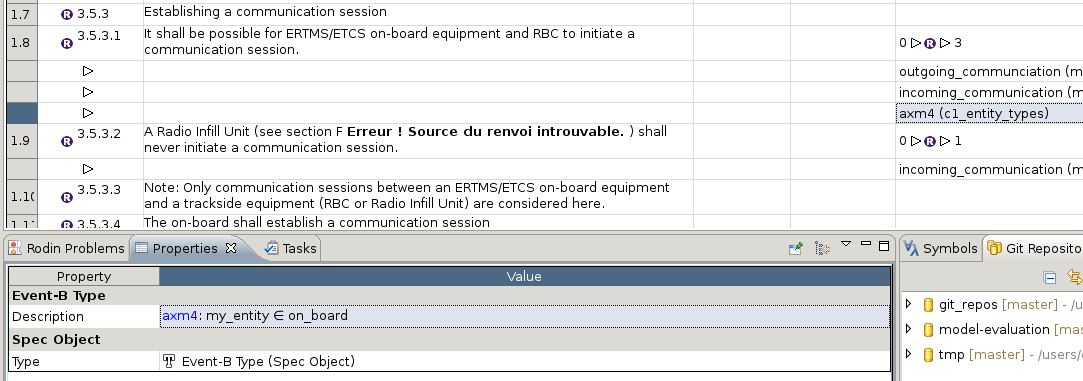
\includegraphics[width=\textwidth]{ProR-Link-View}
  \caption{Properties Window with Element Definition}
  \label{fig:properties-window-element}
\end{figure}


\subsection{How can I animate iUML state machines?}
\label{sec:how-can-i-1}

When a state machine is opened and selected, the buttons to control the
animation and generation of the state machine are activated as shown in
Fig.~\ref{fig:statemachine-anim}. 

\begin{figure}[H]
  \centering
  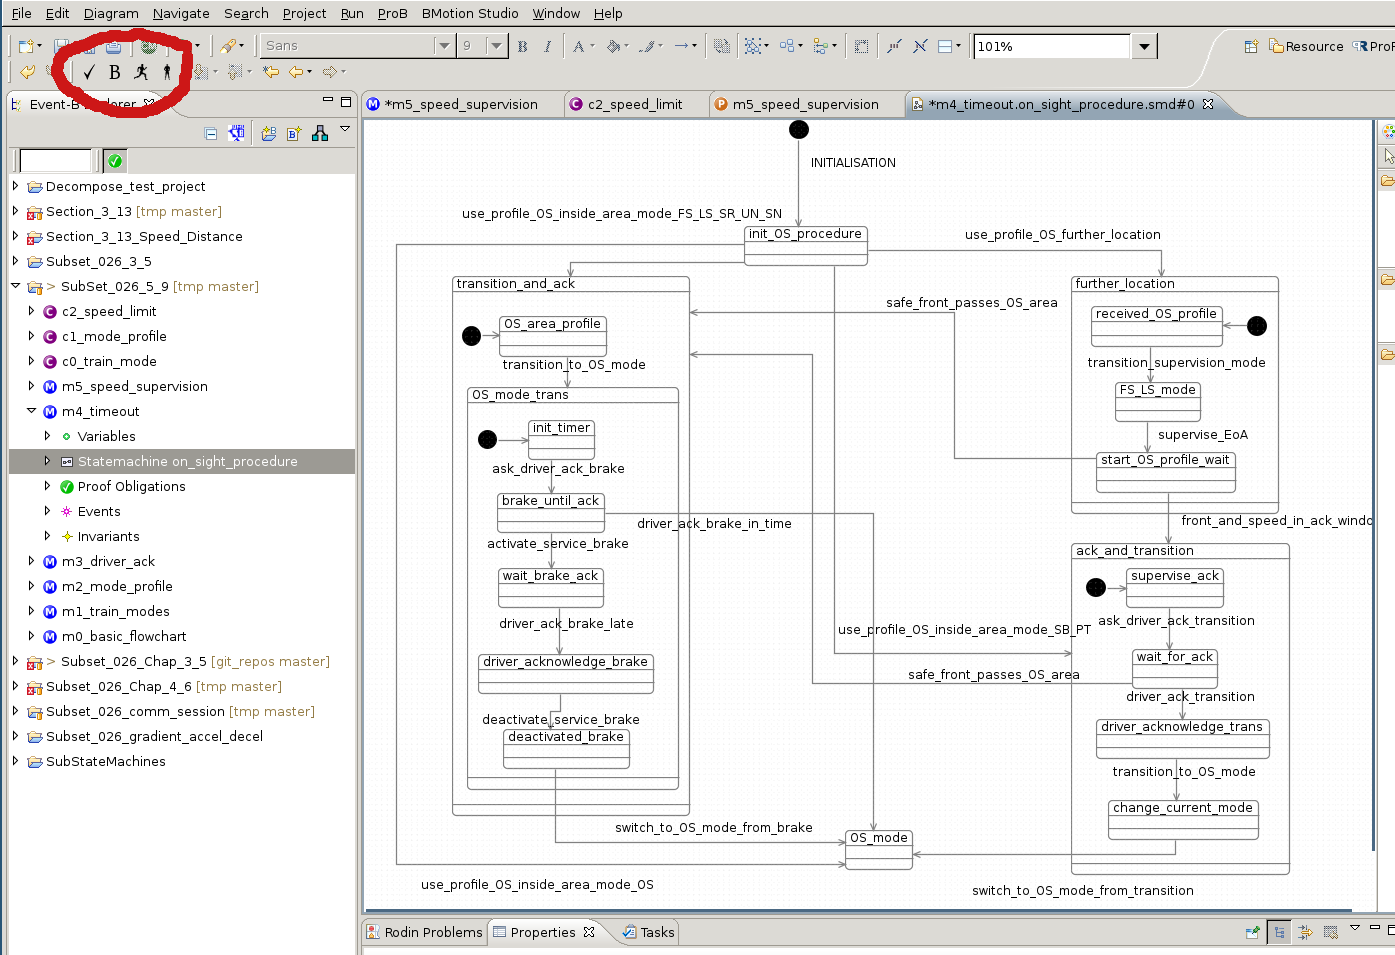
\includegraphics[width=.95\textwidth]{StateMachine1}
  \caption{Opening State Machine for Animation}
  \label{fig:statemachine-anim}
\end{figure}

After selecting the ``Animate With ProB'' button, the state machine is opened in
the animation view as shown in Fig.~\ref{fig:animation-machine}. The active
transitions are highlighted (middle), the activated events are listed and can be executed
by clicking on them (upper left) and the current state of the variables of the
Event-B machines is shown (bottom).

\begin{figure}[H]
  \centering
  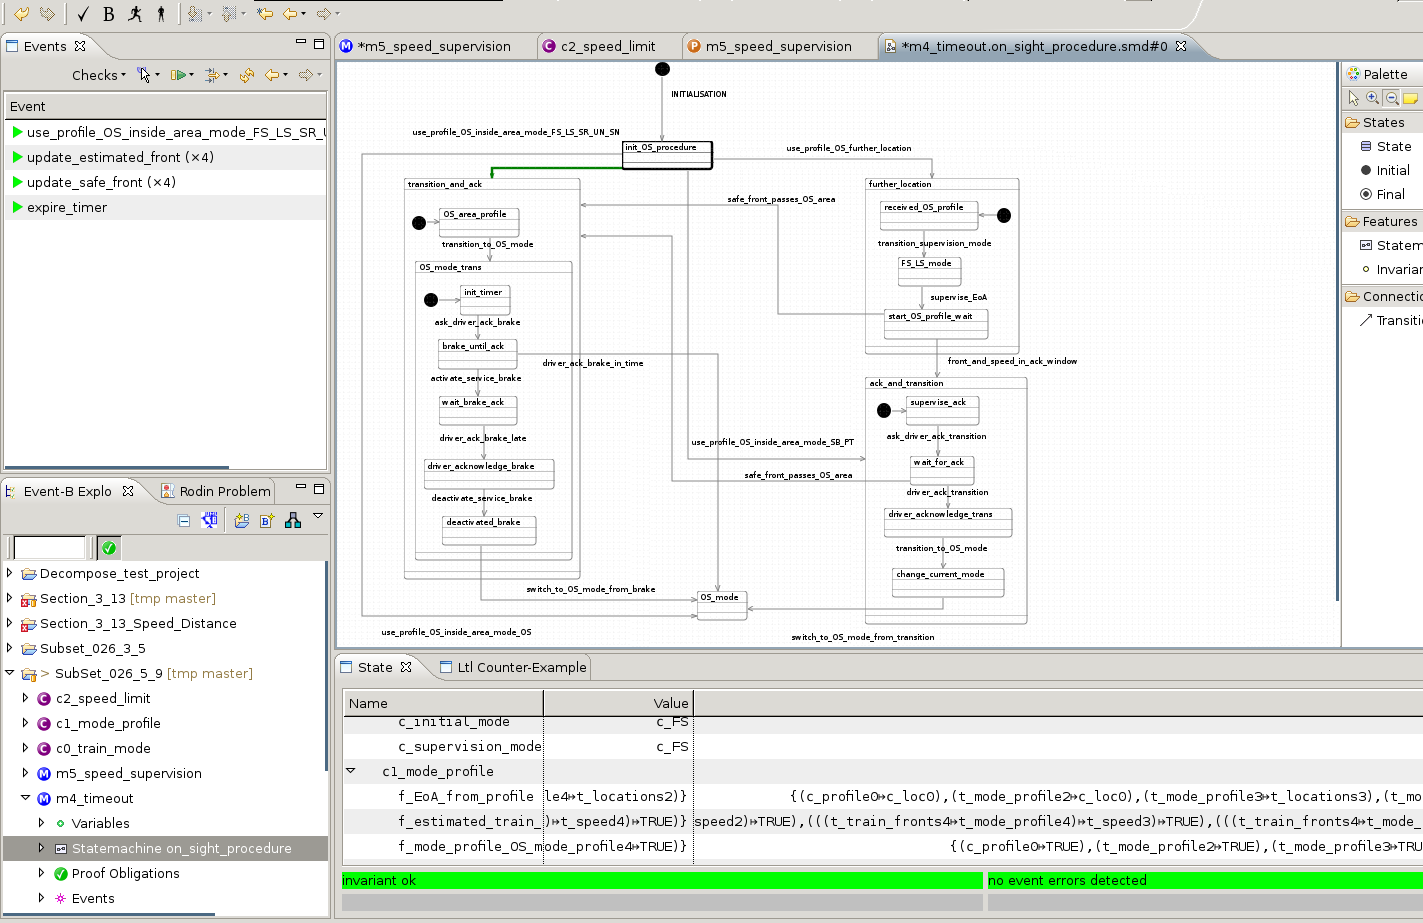
\includegraphics[width=.95\textwidth]{StateMachine2}
  \caption{Animation of State Machine}
  \label{fig:animation-machine}
\end{figure}

\end{document}


%%% Local Variables:
%%% mode: latex
%%% TeX-master: t
%%% End:
